\documentclass{article}
\newtheorem{thm}{Theorem}
\setlength{\oddsidemargin}{0.25in}
\setlength{\textwidth}{6in}
\setlength{\topmargin}{-0.25in}
\setlength{\headheight}{0.3in}
\setlength{\headsep}{0.2in}
\setlength{\textheight}{9in}
\setlength{\footskip}{0.1in}
\usepackage{multirow}
\usepackage{fullpage}
\usepackage{graphicx}
\usepackage{amsthm}
\usepackage{amssymb}
\usepackage{url}
\usepackage{amsfonts}
\usepackage{algpseudocode}
\usepackage{mathtools}
\newcommand{\quotes}[1]{``#1''}
\newcommand{\argmin}{\arg\!\min}
\newcommand{\argmax}{\arg\!\max}

\usepackage{hyperref}
\hypersetup{
    colorlinks=true,
    linkcolor=blue,
    filecolor=magenta,      
    urlcolor=blue,
}

\usepackage{listings}
\usepackage{xcolor} 

\lstset{numbers=left, 
	numberstyle=\tiny, 
	keywordstyle=\color{blue}, 
	commentstyle=\color[cmyk]{1,0,1,0}, 
	frame=single, 
	breaklines, 
	extendedchars=false, 
	xleftmargin=2em,xrightmargin=2em, aboveskip=1em, 
	tabsize=4, 
	showspaces=false 
}

\begin{document}\title{Homework 5\\ Introduction to Data Analysis and Mining \\ Spring 2018\\ CSCI-B 365}         % Enter your title between curly braces
\author{Siyi Xian}        % Enter your name between curly braces
\date{March 25, 2018}          % Enter your date or \today between curly braces
\maketitle
\makeatother     % `@' is restored as a "non-letter" character
\pagestyle{plain}
All the work herein is solely mine.
\section*{Directions}
Please follow the syllabus guidelines in turning in your homework.  I am providing the \LaTeX{} of this document too. This homework is due Sunday, April 8, 2018 10:00p.m. \textbf{OBSERVE THE  TIME}. Absolutely no homework will be accepted after that time. All the work should be your own.  



 
   %%%%%%%%%%%%%%%%%%%%%%%%%%%%%%%%%%%%%%
%                      PROBLEM 1
 %%%%%%%%%%%%%%%%%%%%%%%%%%%%%%%%%%%%%%
 
 
\section*{K-Nearest Neighbors (KNN) Algorithm in Theory}
{\small
\begin{center}
\begin{algorithmic}[1]\label{alg:knn}
\State{\bf ALGORITHM} \texttt{K-nearest neighbors}
\State {\bf INPUT}\begin{itemize}
\item \textsf{training data} $\Delta$
\item \textsf{test data} $\Delta'$  
\item \textsf{distance metric} $d$, i.e., $d:\Delta^2\rightarrow \mathbb{R}_{\geq 0}$ 
\item \textsf{integer} $k$: \textsf{nearest neighbors number}
\end{itemize}
\State {\bf OUTPUT} 
\begin{itemize}
\item \textsf{class label of each} $z \in \Delta' $
\end{itemize}
\For {$z = (\mathbf{x}',y') \in \Delta'$}
\State  \textsf{Compute} $d(\mathbf{x},\mathbf{x}')$, \textsf{the distance between z and every example} $(\mathbf{x},y) \in \Delta$
\State  \textsf{Select} $\Delta_z \subseteq \Delta$, \textsf{the set of closest} $k$ \textsf{training examples to z}
\State \textsf{Voting:}
\begin{itemize}
\item \textsf{majority voting}:
$y' = \argmax_v  \sum_{(\mathbf{x_i},y_i)\in\Delta_z} I(v=y_i)$
\item \textsf{distance-weighted voting}: $y' = \argmax_v  \sum_{(\mathbf{x_i},y_i)\in\Delta_z} w_i \times I(v=y_i)$ \textsf{where} $ w_i = \frac{1}{d(\mathbf{x',x_i})^2}$
\end{itemize}
\EndFor
\end{algorithmic}
\end{center}}

\pagebreak

\section*{K-Fold Cross Validation for Model Selection }

{\small
\begin{center}
\begin{algorithmic}[1]\label{alg:crossValidation}
\State{\bf ALGORITHM} \texttt{k-fold cross validatiaon}
\State {\bf INPUT} \begin{itemize}
\item \textsf{training data} $\Delta = (\mathbf{x_1},y_1),\ldots,(\mathbf{x_m},y_m)$
\item  set of parameter values $\Theta$
\item  learning algorithm $\mathcal{H}$
\item  integer $k$
\end{itemize}
\State {\bf OUTPUT}\begin{itemize}
\item $\theta^* =\argmin_\theta [error(\theta)]$
\item $h_{\theta^*} = \mathcal{H}(\Delta;\theta^*)$ 
\end{itemize}
\State Randomly partition $\Delta$ into $\Delta_1,\ldots,\Delta_k$
\State  \texttt{***} $\Delta_1\cup\Delta_2\ldots \cup\Delta_k = \Delta$ and $\Delta_i \cap \Delta_j = \varnothing$ for $i \neq j \in [1,2,\ldots,k]$
\For{$\theta \in \Theta$}
\For {$i = 1\ldots k$}
\State  \texttt{***}  \textsf{Train a model for each training set}
\State $h_{i,\theta} = \mathcal{H}(\Delta \setminus \Delta_i;\theta)$
\EndFor
\State  \texttt{***}  \textsf{Use the trained models over $\Delta_i$ (test data sets) to evaluate the models for each parameter}
\State error$(\theta)= \frac{1}{k} \sum_{i=1}^{k} \mathcal{L}_{\Delta_i} (h_{i,\theta})$
\EndFor
\end{algorithmic}
\end{center}}
%%%%%%%%%%%%%%%%%%%%%%%%%%%%%%%%%%%%%%
In this homework, you are asked to train several classifiers  using $k$-nearest neighbors (KNN) and  naive bayes  algorithms over  car evaluation and credit approval data sets.  The links for the data sets are provided below:
  
 \begin{itemize}
\item \href{https://archive.ics.uci.edu/ml/datasets/car+evaluation}{Car Evaluation Data Set}
\item \href{https://archive.ics.uci.edu/ml/datasets/Credit+Approval}{Credit Approval Data Set }
\end{itemize}

%%%%%%%%%%%%%%%%%%%%%%%%%%%%%%%%%%%%%%
\section*{Problem 1: $K$-Fold Cross Validation [20 points]}

Create $5$ training and $5$ test data sets from each data set using  $5$-fold cross validation and save these $20$ files. You will use these data sets to answer the rest of the questions. You are allowed to use R packages for $k$- fold cross validation. However,\textit{ students who implement it will receive $15$ extra points from this question}.

\begin{verbatim}
Please see specific code in crossValidation.R (Starts from line 163).
\end{verbatim}

%%%%%%%%%%%%%%%%%%%%%%%%%%%%%%%%%%%%%%
\section*{Problem 2: $K$-Nearest Neighbors (KNN)[40 points]} 

\textbf{2.1}  Implement KNN algorithm with two different distance functions. You can either use existing distance functions, i.e., Euclidean  or design your own.
\begin{verbatim}
Please see specific code in knn.R (Starts from line 26).
\end{verbatim}
\pagebreak
\textbf{2.2}  Use the data sets created in problem 1 to determine the optimal $k$  over each data set for KNN algorithm. First, pick 5  different $k$ values and then calculate average error rate of  KNN classifiers over test data tests  for each $k$ to find the optimal $k$ for each data set and distance function. Report the average error rate for each $k$, distance function and data set.  What are the optimal $k$ and distance function for each data set?
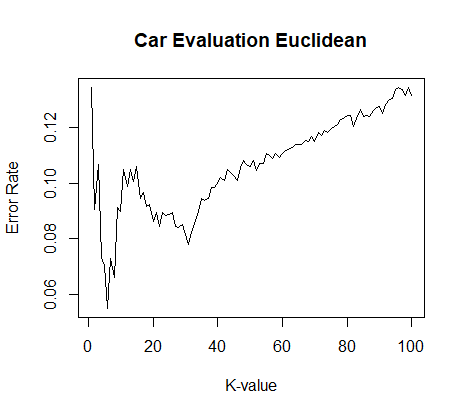
\includegraphics[width=8cm]{CarEvaluationEuclidean.PNG}
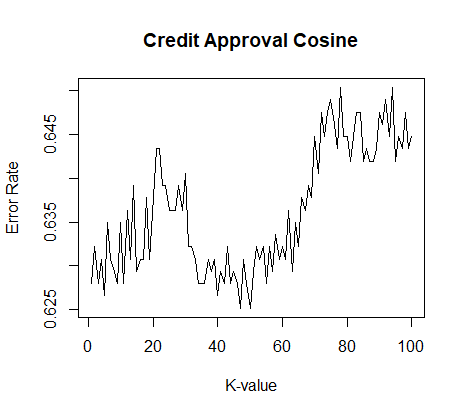
\includegraphics[width=8cm]{CarEvaluationCosine.PNG}
\\
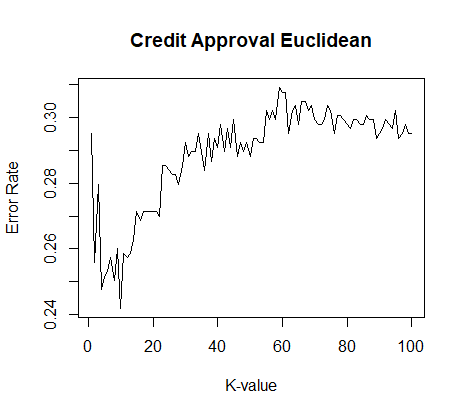
\includegraphics[width=8cm]{CreditApprovalEuclidean.PNG}
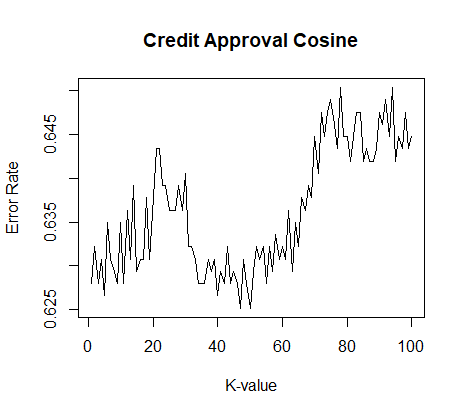
\includegraphics[width=8cm]{CreditApprovalCosine.PNG}
\begin{verbatim}
Acoording to the graph above, we can decided that:
	1. For both data sets, Euclidean will be a better way to calculate distance that Consine.
	2. For Car Evaluation Data Set, when K = 7, the error rate will be smallest.
	3. For Credit Approval Data Set, when K = 11, the error rate will be the best one to choose.

For specofoc code, please look at the end of crossValidation.R (Starts from line 206).
\end{verbatim}
\pagebreak
\textbf{2.3} Use the KNN package in R  to validate your results from question 2.2.
\\
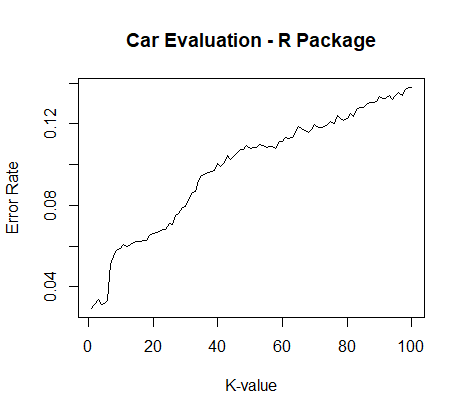
\includegraphics[width=8cm]{CarEvaluation_R.PNG}
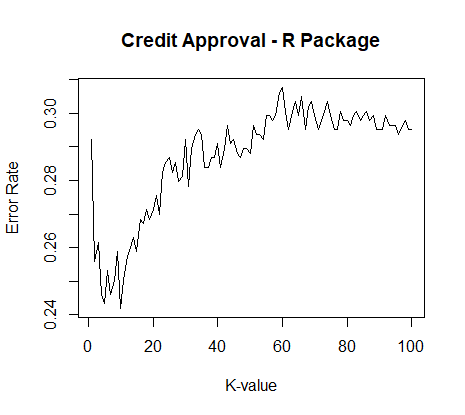
\includegraphics[width=8cm]{CreditApproval_R.PNG}
\begin{verbatim}
    When using R pakage, knn will be more efficet due to the run time is much more 
smaller. However, for the sesualt, it is similar. We will better to choose 2 or 5 for 
K value in Car Evaluation Data Set. And as for Credit Approval Data Set, we will going 
to choose K = 11 too. On the other hand, the fluctuation is also similar

Please see specific code in knnValidation.R.
\end{verbatim}
\pagebreak
 %%%%%%%%%%%%%%%%%%%%%%%%%%%%%%%%%%%%%%
\section*{Problem 3: Naive Bayes Classifier vs. $K$-Nearest Neighbors [20 points]} 

In this question, you are  first asked to train Naive Bayes classifiers to find the optimal Naive Bayes model for  car evaluation and credit approval data sets. Second, you will  compare your optimal KNN and Naive Bayes models over  car evaluation and credit approval data sets.  Answer the following questions:

\begin{enumerate}
\item[\textbf{3.1}] Train Naive Bayes classifiers over training data sets and test each classifier over corresponding  test data.  Report the error rates  of the classifiers  in a figure. Create one figure for car evaluation  data set and  another one for credit approval data set. You are allowed to use R packages for Naive Bayes algorithm.
\begin{lstlisting}[language=R]
# Please see detailed code in naiveBayes.R file
> CarEvaluationErrorRates
[1] 0.1987458
> CreditApprovalErrorRates
[1] 0.2106917
\end{lstlisting}
\item[\textbf{3.2}] Pick the optimal Naive Bayes classifiers (one for  car evaluation  data set and  another one for credit approval data set.) from question 3.1 and compare them with your best KNN models from question 2. Discuss the performances of the optimal classifiers over car evaluation and credit approval data sets, i.e, which one performed better? 
\begin{verbatim}
    For Car Evaluation Data Set, our best error rate is arround 0.04. So for here, 
KNN can do a better job that Naive Bayes. When we comes to Credit Approval Data Set, 
the minimum error rate using KNN is 0.24. It is larger than the error rate when doing 
Naive Bayes. In conclusion, we can find out that the efficence for different algorithm 
is based on database. Thus, we need to figure out choosing algorithm after studying 
data set.
\end{verbatim}
\end{enumerate}
\pagebreak
\section*{Problem 4 [10 points]} 
\begin{itemize}
	\item [\textbf{7.}]Consider the data set shown in Table 5.1
	\begin{itemize}
		\item [\textbf{(a)}]Estimate the conditional probabilities for $P(A|+)$, $P(B|+)$, $P(C|+)$,
		$P(A|-)$, $P(B|-)$, and $P(C|-)$.
		\begin{itemize}
			\item  $P(A = 1|+) = \dfrac{3}{5} = 0.6$
			\item  $P(A = 0|+) = \dfrac{2}{5} = 0.4$
			\item  $P(B = 1|+) = \dfrac{1}{5} = 0.2$
			\item  $P(B = 0|+) = \dfrac{4}{5} = 0.8$
			\item  $P(C = 1|+) = \dfrac{4}{5} = 0.8$
			\item  $P(C = 0|+) = \dfrac{1}{5} = 0.2$
			\item  $P(A = 1|-) = \dfrac{2}{5} = 0.4$
			\item  $P(A = 0|-) = \dfrac{3}{5} = 0.6$
			\item  $P(B = 1|-) = \dfrac{2}{5} = 0.4$
			\item  $P(B = 0|-) = \dfrac{3}{5} = 0.6$
			\item  $P(C = 1|-) = \dfrac{0}{5} = 0$
			\item  $P(C = 0|-) = \dfrac{5}{5} = 1$
		\end{itemize}
		\item [\textbf{(b)}]Use the estimate of conditional probabilities given in the previous question
		to predict the class label for a test sample $(A = 0,B = 1, C = 0)$ using the na\"{\i}ve Bayes approach.\\
		Let $ P(A = 0,B = 1, C = 0) = K $.\\
		$  P(+|A = 0,B = 1, C = 0) $\\
		$= \dfrac{ P(+|A = 0,B = 1, C = 0)\times P(+)}{ P(A = 0,B = 1, C = 0)}$\\
		$=\dfrac{P(+|A = 0,B = 1, C = 0)\times P(+)}{K}$\\
		$=\dfrac{P(A = 0|+)P(B = 1|+)P(C = 0|+) \times P(+)}{K}$\\
		$=\dfrac{0.4 \times 0.2 \times 0.2 \times 0.5}{K}$\\
		$=\dfrac{0.008}{K}$\\
		$  P(-|A = 0,B = 1, C = 0) $\\
		$= \dfrac{ P(-|A = 0,B = 1, C = 0)\times P(-)}{ P(A = 0,B = 1, C = 0)}$\\
		$=\dfrac{P(-|A = 0,B = 1, C = 0)\times P(-)}{K}$\\
		$=\dfrac{P(A = 0|-)P(B = 1|-)P(C = 0|-) \times P(-)}{K}$\\
		$=\dfrac{0.6 \times 0.4 \times 0 \times 0.5}{K}$\\
		$=0$\\
		\begin{verbatim}
		We will going to choose +
		\end{verbatim}
		\pagebreak
		\item[\textbf{(c).}] Estimate the conditional probabilities using the m-estimate approach, with $p = 1/2$ and $m = 4$.
		\begin{itemize}
			\item  $P(A = 1|+) = \dfrac{3 + 2}{5 + 4} = \dfrac{5}{9}$
			\item  $P(A = 0|+) = \dfrac{2 + 2}{5 + 4} = \dfrac{4}{9}$
			\item  $P(B = 1|+) = \dfrac{1 + 2}{5 + 4} = \dfrac{3}{9}$
			\item  $P(B = 0|+) = \dfrac{4 + 2}{5 + 4} = \dfrac{6}{9}$
			\item  $P(C = 1|+) = \dfrac{4 + 2}{5 + 4} = \dfrac{6}{9}$
			\item  $P(C = 0|+) = \dfrac{1 + 2}{5 + 4} = \dfrac{3}{9}$
			\item  $P(A = 1|-) = \dfrac{2 + 2}{5 + 4} = \dfrac{4}{9}$
			\item  $P(A = 0|-) = \dfrac{3 + 2}{5 + 4} = \dfrac{5}{9}$
			\item  $P(B = 1|-) = \dfrac{2 + 2}{5 + 4} = \dfrac{4}{9}$
			\item  $P(B = 0|-) = \dfrac{3 + 2}{5 + 4} = \dfrac{5}{9}$
			\item  $P(C = 1|-) = \dfrac{0 + 2}{5 + 4} = \dfrac{2}{9}$
			\item  $P(C = 0|-) = \dfrac{5 + 2}{5 + 4} = \dfrac{7}{9}$
		\end{itemize}
		\item[\textbf{(d)}] Repeat part \textbf{(b)} using the conditional probabilities given in part \textbf{(c)}.
		Let $ P(A = 0,B = 1, C = 0) = K $.\\
		$  P(+|A = 0,B = 1, C = 0) =\dfrac{0.0247}{K}$\\
		$  P(-|A = 0,B = 1, C = 0) =\dfrac{0.0549}{K}$\\
		\begin{verbatim}
		We will going to choose -
		\end{verbatim}
		\item[\textbf{(e)}] Compare the two methods for estimating probabilities. Which method is better and why?
		\begin{verbatim}
		The m-estimate approach is better, becasue it can avoid 0 whihc happend in naive 
		Bayes approach.
		\end{verbatim}
	\end{itemize}
\end{itemize}

\pagebreak
 %%%%%%%%%%%%%%%%%%%%%%%%%%%%%%%%%%%%%%
%                   EXTRA CREDIT
 %%%%%%%%%%%%%%%%%%%%%%%%%%%%%%%%%%%%%%
  \section*{Extra Credit [30 points]} 
\begin{itemize}
%\item From textbook, Chapter 5 exercises 8, 17 (Pages 318 $\&$ 322) \textbf{[15 points}]
\item Problem 1: $K$-fold cross validation implementation  \textbf{[15 points}]
\begin{verbatim}
Please see code in crossValidation.R
\end{verbatim}
\end{itemize}




%%%%%%%%%%%%%%%%%%%%%%%%%%%%%%%%%%%%%%
\section*{What to Turn-in}
 Submit a .zip file that includes the files below. Name the .zip  file as \quotes{usename-section number}, i.e., hakurban-B365.


\begin{itemize}
\item The *tex and *pdf of the written answers to this document.
\item *\texttt{R}files for:
\begin{itemize}
\item Question 1: \textsf{crossValidation.R}, output of cross validation: training  and test data sets 
\item Question 2.1: \textsf{knn.R}, Question 2.3: \textsf{knnValidation.R}
\item Question 3: \textsf{naiveBayes.R}
\end{itemize} 
\item A README file that explains how to run your code and other files in the folder
\end{itemize}




\end{document}


